\section{Ichki energiya.}



\begin{enumerate}

\item Jismning (moddaning) ichki energiyasi deganda, nimani tushunamiz:
\begin{enumerate}
\item $1$ kg massali moddaning temperaturasini $1$ gradusga oshirish uchun sarflangan issiqlik miqdori;
\item issiqlik almashishida jism olgan yoki uzatgan issiqlik miqdori;
\item moddaning temperaturasini $1$ gradusga oshirish uchun sarflangan issiqlik miqdori;
\item jismni tashkil etuvchi barcha molekulalarning kinetik va o‘zaro ta’sir potensial energiyalarining yig‘indisi.
\end{enumerate}
\begin{enumerate}[label=\Alph*)]
\item 4
\item 3
\item 2
\item 1

\end{enumerate}

\item Temperaturasi $361$ K bo‘lgan $4$ mol bir atomli gazning ichki energiyasini toping (kJ).
\begin{enumerate}[label=\Alph*)]
\item 20
\item 18
\item 30
\item 38

\end{enumerate}

\item Ichki energiyasi $20$ kJ bo‘lgan $6$ mol bir atomli gazning temperaturasini toping (K).
\begin{enumerate}[label=\Alph*)]
\item 267,4
\item 607,5
\item 165,9
\item 982,8

\end{enumerate}

\item Temperaturasi $127^\circ$C bo‘lgan bir atomli gazning ichki energiyasi $74,79$ kJ ga teng. Gazning modda miqdorini toping (mol).
\begin{enumerate}[label=\Alph*)]
\item 28
\item 18
\item 30
\item 15

\end{enumerate}

\item $1$ mol miqdordagi bir atomli ideal gazning ichki energiyasini aniqlovchi ifodani toping:
\begin{enumerate}
\item $3kT/2$
\item $3RT/2$
\item $3N_AkT/2$
\item $kT/2$
\end{enumerate}
\begin{enumerate}[label=\Alph*)]
\item 1
\item 1 va 2
\item 2 va 3
\item 4

\end{enumerate}

\item $1$ mol bir atomli ideal gaz molekulalarining o‘rtacha kinetik energiyalari yig‘indisi qaysi ifodada to‘g‘ri ko‘rsatilgan?
\begin{enumerate}[label=\Alph*)]
\item $E_k=3kT$
\item $E_k=3RT/2$
\item $E_k=3kT/2$
\item $E_k=3RT$

\end{enumerate}

\item Temperaturasi $-73^\circ$C bo‘lgan bir mol bir atomli ideal gazning ichki energiyasini toping (J).
\begin{enumerate}[label=\Alph*)]
\item 1246
\item 1662
\item 2077
\item 2493

\end{enumerate}

\item Rasmda bir atomli ideal gaz ichki energiyasining absolut temperaturaga bog‘lanish grafigi tasvirlangan. Grafikdan foydalanib, gazning modda miqdorini (mol) ni aniqlang. $R=8,31$ J/(mol$\cdot$K).

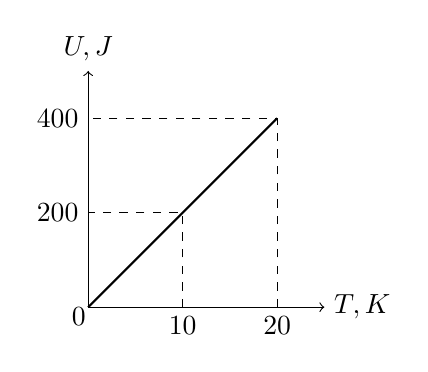
\begin{tikzpicture}[scale=0.6]
    % Koordinata o'qlari
    \draw[->] (0,0) -- (5,0) node[right] {$T, \text{K}$};
    \draw[->] (0,0) -- (0,5) node[above] {$U, \text{J}$};
    \node at (-0.2,-0.2) {$0$};

    % Grafik chizig'i
    \draw[thick] (0,0) -- (4,4);

    % Punktir chiziqlar va qiymatlar
    \draw[dashed] (2,0) node[below] {$10$} -- (2,2) -- (0,2) node[left] {$200$};
    \draw[dashed] (4,0) node[below] {$20$} -- (4,4) -- (0,4) node[left] {$400$};
\end{tikzpicture}

\begin{enumerate}[label=\Alph*)]
\item 0,5
\item 1,6
\item 10
\item 16

\end{enumerate}

\item $225$ K temperaturali bir atomli gaz berilgan. Undagi molekulalar soni $7\cdot10^{24}$ ta bo‘lsa, gaz ichki energiyasini toping (kJ).
\begin{enumerate}[label=\Alph*)]
\item 25,8
\item 21,8
\item 32,6
\item 28,1

\end{enumerate}

\item Massasi $200$ g bo‘lgan geliy gazining temperaturasi $500$ K ga teng. Uning ichki energiyasini toping (kJ). $\mu=4$ g/mol.
\begin{enumerate}[label=\Alph*)]
\item 564,45
\item 345,52
\item 876,065
\item 311,625

\end{enumerate}

\item Temperaturasi $-73^\circ$C va ichki energiyasi $2493$ J bo‘lgan geliy gazining massasini aniqlang (g).
\begin{enumerate}[label=\Alph*)]
\item 3
\item 4
\item 6
\item 17

\end{enumerate}

\item Ichki energiyasi $50$ kJ bo‘lgan neon gazining massasi $1,2$ kg ga teng. Uning temperaturasi toping (K). $\mu=20$ g/mol.
\begin{enumerate}[label=\Alph*)]
\item 64,45
\item 35,26
\item 66,85
\item 11,15

\end{enumerate}

\item Ichki energiyasi $100$ kJ bo‘lgan bir atomli gazning massasi $334,27$ g va temperaturasi $327^\circ$C ga teng. Uning molyar massasini toping (g/mol).
\begin{enumerate}[label=\Alph*)]
\item 25
\item 21
\item 32
\item 28

\end{enumerate}

\item $10$ litr hajmli bir atomli gazning bosimi $40$ kPa ga teng. Uning ichki energiyasini toping (J).
\begin{enumerate}[label=\Alph*)]
\item 250
\item 420
\item 130
\item 600

\end{enumerate}

\item Bosimi $24$ Pa bo‘lgan bir atomli gazning ichki energiyasi $36$ J ga teng. Uning hajmini toping (m$^3$).
\begin{enumerate}[label=\Alph*)]
\item 1
\item 2
\item 3
\item 4

\end{enumerate}

\item Idishning hajmi $2$ litr, undagi geliyning bosimi $10$ kPa. Gazning ichki energiyasi (J) nimaga teng?
\begin{enumerate}[label=\Alph*)]
\item 20
\item 60
\item 30
\item 45

\end{enumerate}

\item Agar bir atomli ideal gazning hajmi $2$ m$^3$ va ichki energiyasi $1500$ J bo‘lsa, uning bosimi qanday (Pa)?
\begin{enumerate}[label=\Alph*)]
\item 500
\item 1500
\item 1000
\item 300

\end{enumerate}

\item Bosimi $4\cdot10^5$ Pa bo‘lgan $1$ m$^3$ bir atomli ideal gaz molekulalarining kinetik energiyalari yig‘indisini toping (J).
\begin{enumerate}[label=\Alph*)]
\item $2\cdot10^5$
\item $6\cdot10^5$
\item $8\cdot10^5$
\item $12\cdot10^5$

\end{enumerate}

\item Molekulalarining o‘rtacha kvadratik tezligi $500$ m/s bo‘lgan $20$ g massali bir atomli gazning ichki energiyasi necha Joul bo‘ladi?
\begin{enumerate}[label=\Alph*)]
\item 50
\item 250
\item 200
\item 2500

\end{enumerate}

\item Bosimlari va hajmlari bir xil bo‘lgan kislorod va vodorod gazlarining $U_1$ va $U_2$ ichki energiyalarini solishtiring.
\begin{enumerate}[label=\Alph*)]
\item $U_1=32U_2$
\item $U_1=16U_2$
\item $U_1=U_2$
\item $U_2=16U_1$

\end{enumerate}

\item Bosimlari $p_1=2p_2$, hajmlari $V_2=2V_1$ bo‘lgan bir atomli ideal gazlarning ichki energiyalarini taqqoslang.
\begin{enumerate}[label=\Alph*)]
\item $U_1=4U_2$
\item $U_1=2U_2$
\item $U_1=U_2$
\item $U_2=2U_1$

\end{enumerate}

\item Argon va geliy gazlari bir xil massaga ega bo‘lib, bir xil sharoitda turibdi. Ularning ichki energiyalarini taqqoslang. ($\mu_{Ar}=40$ g/mol, $\mu_{He}=4$ g/mol)
\begin{enumerate}[label=\Alph*)]
\item geliyniki 10 marta katta.
\item argonniki 10 marta katta.
\item barobar.
\item argonniki 4 marta kichik.

\end{enumerate}

\item Temperaturalari bir xil bo‘lgan teng massali geliy va argonning ichki energiyalari nisbati qanday bo‘ladi? Geliyning molyar massasi 4 g/mol, argonniki 40 g/mol.
\begin{enumerate}[label=\Alph*)]
\item 1
\item 2
\item 10
\item 1/4

\end{enumerate}

\item Bir atomli gaz molekulalarining konsentratsiyasi $n$ bo‘lsa, $T$ haroratda $V$ hajmni egallagan gazning ichki energiyasi qanday bo‘ladi?
\begin{enumerate}[label=\Alph*)]
\item $\frac{3mV}{2\mu}RT$
\item $\frac{3nV}{2}RT$
\item $\frac{3m}{2\mu}RT$

\end{enumerate}

\item Ideal gaz $pV$ diagrammada qaysi nuqtaga mos keluvchi holatda eng katta ichki energiyaga ega bo‘ladi?

\begin{tikzpicture}[scale=0.6]
    % Koordinata o'qlari
    \draw[->] (0,0) -- (5,0) node[right] {$V$};
    \draw[->] (0,0) -- (0,5) node[above] {$p$};
    \node at (-0.3,-0.3) {$O$};

    % Nuqtalar va ularning raqamlari
    \filldraw (1,1) circle (1.5pt) node[right, xshift=2pt] {$1$};
    \filldraw (1.2,3.5) circle (1.5pt) node[left, xshift=-2pt] {$2$};
    \filldraw (4,3.5) circle (1.5pt) node[left, xshift=-2pt] {$3$};
    \filldraw (3.8,1) circle (1.5pt) node[right, xshift=2pt] {$4$};
    \filldraw (2.5,2.2) circle (1.5pt) node[right, xshift=2pt] {$5$};
\end{tikzpicture}

\begin{enumerate}[label=\Alph*)]
\item 1
\item 2
\item 3
\item 4

\end{enumerate}

\item Grafikda $p$–$V$ koordinatalarda ideal gaz holatining o‘zgarishi ifodalangan. Gazning ichki energiyasiga qaysi nuqtasiga mos holatda eng katta qiymatga erishadi?

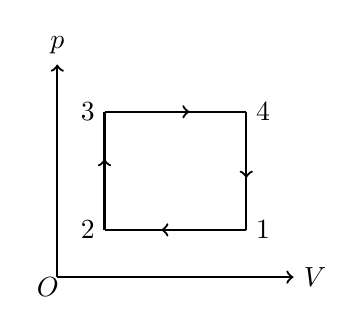
\begin{tikzpicture}[scale=0.6]
    % Koordinata o'qlari
    \draw[->, thick] (0,0) -- (5,0) node[right] {$V$}; % V o'qi
    \draw[->, thick] (0,0) -- (0,4.5) node[above] {$p$}; % p o'qi
    \node at (-0.2,-0.2) {$O$}; % Koordinata boshi

    % Siklning to'rtta uchi (1, 2, 3, 4 nuqtalar)
    % 2-nuqta (1,1), 3-nuqta (1,3.5), 4-nuqta (4,3.5), 1-nuqta (4,1)

    % 2 dan 3 ga (izoxora, bosim ortishi)
    \draw[thick] (1,1) -- (1,3.5);
    \draw[->, thick] (1,1) -- (1,2.5); % Yo'nalish strelkasi
    \node[left] at (1,1) {$2$};
    \node[left] at (1,3.5) {$3$};

    % 3 dan 4 ga (izobara, hajm ortishi)
    \draw[thick] (1,3.5) -- (4,3.5);
    \draw[->, thick] (1,3.5) -- (2.8,3.5); % Yo'nalish strelkasi
    \node[right] at (4,3.5) {$4$};

    % 4 dan 1 ga (izoxora, bosim kamayishi)
    \draw[thick] (4,3.5) -- (4,1);
    \draw[->, thick] (4,3.5) -- (4,2.1); % Yo'nalish strelkasi
    \node[right] at (4,1) {$1$};

    % 1 dan 2 ga (izobara, hajm kamayishi)
    \draw[thick] (4,1) -- (1,1);
    \draw[->, thick] (4,1) -- (2.2,1); % Yo'nalish strelkasi
\end{tikzpicture}

\begin{enumerate}[label=\Alph*)]
\item 1
\item 2
\item 3
\item 4
\end{enumerate}

\item Ideal gaz holatining o‘zgarish diagrammasida qaysi nuqtaga ichki energiyaning eng katta qiymati mos keladi?

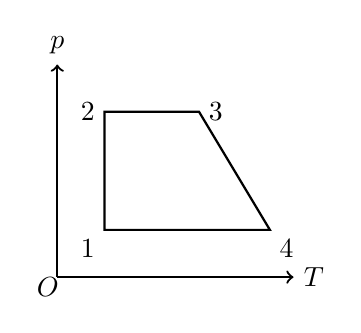
\begin{tikzpicture}[scale=0.6]
    % Koordinata o'qlari
    \draw[->, thick] (0,0) -- (5,0) node[right] {$T$};
    \draw[->, thick] (0,0) -- (0,4.5) node[above] {$p$};
    \node at (-0.2,-0.2) {$O$};

    % Sikl nuqtalari koordinatalari
    \coordinate (1) at (1,1);
    \coordinate (2) at (1,3.5);
    \coordinate (3) at (3,3.5);
    \coordinate (4) at (4.5,1);

    % Sikl chiziqlari
    \draw[thick] (1) -- (2) -- (3) -- (4) -- cycle;

    % Nuqtalarni raqamlash
    \node[below left] at (1) {1};
    \node[left] at (2) {2};
    \node[right] at (3) {3};
    \node[below right] at (4) {4};
\end{tikzpicture}

\begin{enumerate}[label=\Alph*)]
\item 1
\item 2
\item 3
\item 4

\end{enumerate}

\item Ideal gaz holatining o‘zgarish diagrammasidagi qaysi nuqtaga ichki energiyaning eng kichik qiymati mos keladi?

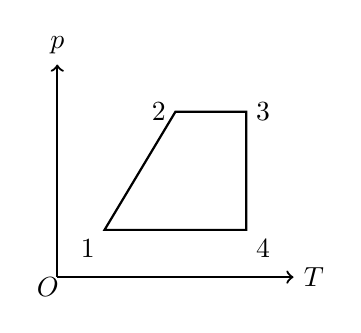
\begin{tikzpicture}[scale=0.6]
    % Koordinata o'qlari
    \draw[->, thick] (0,0) -- (5,0) node[right] {$T$};
    \draw[->, thick] (0,0) -- (0,4.5) node[above] {$p$};
    \node at (-0.2,-0.2) {$O$};

    % Sikl nuqtalari koordinatalari
    \coordinate (1) at (1,1);
    \coordinate (2) at (2.5,3.5);
    \coordinate (3) at (4,3.5);
    \coordinate (4) at (4,1);

    % Sikl chiziqlari
    \draw[thick] (1) -- (2) -- (3) -- (4) -- cycle;

    % Nuqtalarni raqamlash
    \node[below left] at (1) {1};
    \node[left] at (2) {2};
    \node[right] at (3) {3};
    \node[below right] at (4) {4};
\end{tikzpicture}

\begin{enumerate}[label=\Alph*)]
\item 1
\item 2
\item 3
\item 4

\end{enumerate}

\item $p$–$\rho$ koordinatalarda gazning holatini ifodalovchi nuqtalar berilgan ($p$ – bosim, $\rho$ – zichlik). Bu nuqtalardan qaysi birida gazning ichki energiyasi eng katta bo‘ladi?

\begin{tikzpicture}[scale=0.6]
    % Koordinata o'qlari
    \draw[->, thick] (0,0) -- (5,0) node[right] {$\rho$};
    \draw[->, thick] (0,0) -- (0,4) node[above] {$p$};

    % Nuqtalarni joylashtirish
    \filldraw (1.5,3) circle (1.5pt) node[left, xshift=-2pt] {1};
    \filldraw (4,3) circle (1.5pt) node[right, xshift=2pt] {2};
    \filldraw (1.5,1) circle (1.5pt) node[left, xshift=-2pt] {3};
    \filldraw (4,1) circle (1.5pt) node[right, xshift=2pt] {4};
\end{tikzpicture}

\begin{enumerate}[label=\Alph*)]
\item 1
\item 4
\item 2
\item 3

\end{enumerate}

\item Boshlang‘ich temperaturasi $250$ K va oxirgi temperaturasi $400$ K bo‘lgan $12$ g geliyning ichki energiya o‘zgarishini toping (J).
\begin{enumerate}[label=\Alph*)]
\item 5421,05
\item 1894,04
\item 2345,54
\item 5609,25

\end{enumerate}

\item Temperaturasi $400$ K bo‘lgan $3$ mol argon gaziga issiqlik berib, temperaturasini $460$ K ga yetkazdi. Uning ichki energiya o‘zgarishini toping (J).
\begin{enumerate}[label=\Alph*)]
\item 5645,5
\item 2243,7
\item 9804,3
\item 5670,1

\end{enumerate}

\item $2$ mol geliy $20^\circ$C dan $-80^\circ$C gacha sovitilganda, uning ichki energiyasi necha kJ kamayadi?
\begin{enumerate}[label=\Alph*)]
\item 8,31
\item 25
\item 2,5
\item 16,62

\end{enumerate}

\item $4\cdot10^{23}$ ta molekulaga ega bo‘lgan bir atomli ideal gazning temperaturasi $100$ K ga ortganda, ichki energiyasi necha J ga o‘zgaradi? $N_A=6\cdot10^{23}$ mol$^{-1}$.
\begin{enumerate}[label=\Alph*)]
\item 8,31
\item 38,1
\item 415
\item 831

\end{enumerate}

\item Hajmi $80$ l bo‘lgan ballonda bir atomli ideal gaz bor. Uning bosimi $150$ kPa dan $220$ kPa gacha oshsa ichki energiyasi qancha oshadi (kJ)?
\begin{enumerate}[label=\Alph*)]
\item 8,4
\item 3,8
\item 6,6
\item 9,7

\end{enumerate}

\item Bosimi $200$ kPa bo‘lgan bir atomli ideal gazning hajmi izobarik ravishda $75$ l dan $195$ l gacha ortdi. Uning ichki energiyasi o‘zgarishini toping (kJ)?
\begin{enumerate}[label=\Alph*)]
\item 45
\item 93
\item 84
\item 36

\end{enumerate}

\item Bir atomli ideal gazga izobarik siqilganda, gaz izobar ravishda $0,05$ m$^3$ ga kengaydi. Agar gazning bosimi $10^5$ Pa bo‘lsa, gazning ichki energiyasi necha kJ ortgan?
\begin{enumerate}[label=\Alph*)]
\item 5,5
\item 8
\item 7,5
\item 9
\end{enumerate}

\item Gazning izotermik kengayishida uning ichki energiyasi qanday o‘zgaradi?
\begin{enumerate}[label=\Alph*)]
\item ortadi
\item o‘zgarmaydi
\item kamayadi
\item ichki energiya ixtiyoriy bo‘lishi mumkin

\end{enumerate}

\item Metall silindrdagi gaz porshen bilan izotermik siqilganda, uning hajmi $5$ marta kamaydi. Bunda gazning ichki energiyasi qanday o‘zgaradi?
\begin{enumerate}[label=\Alph*)]
\item 5 marta ortadi
\item o‘zgarmaydi
\item 5 marta kamayadi
\item 2,5 marta ortadi

\end{enumerate}

\item Ideal gaz bosimi va absolut temperaturasi $2$ marta oshsa, uning ichki energiyasi qanday o‘zgaradi?
\begin{enumerate}[label=\Alph*)]
\item o‘zgarmaydi
\item 2 marta kamayadi
\item 2 marta oshadi
\item 4 marta kamayadi

\end{enumerate}

\item Ideal gaz bir holatdan ikkinchi holatga 3 xil usul bilan o‘tkazildi: $1\to a\to 2$, $1\to b\to 2$, $1\to c\to 2$. Bu usullarda gazning ichki energiya o‘zgarishini taqqoslang.

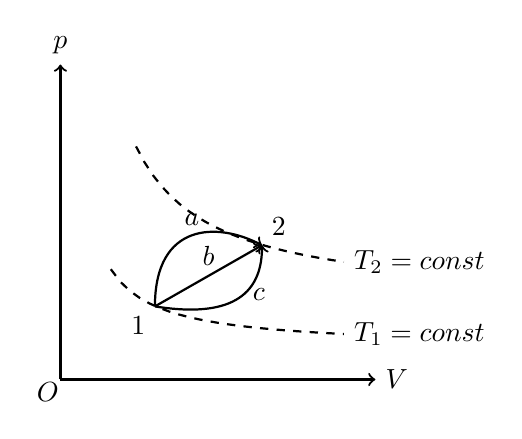
\begin{tikzpicture}[scale=0.8]
    % O'qlar
    \draw[->, thick] (0,0) -- (5,0) node[right] {$V$};
    \draw[->, thick] (0,0) -- (0,5) node[above] {$p$};
    \node at (-0.2,-0.2) {$O$};

    % Izotermalar (punktir)
    \draw[dashed, thick, domain=0.8:4.5] plot (\x, {1/\x + 0.5}) node[right] {$T_1=\text{const}$};
    \draw[dashed, thick, domain=1.2:4.5] plot (\x, {3/\x + 1.2}) node[right] {$T_2=\text{const}$};

    % Nuqtalar koordinatalari
    \coordinate (1) at (1.5, 1.16);
    \coordinate (2) at (3.2, 2.13);

    % Yo'llar (a, b, c)
    \draw[thick, ->] (1) .. controls (1.5, 2.5) and (2.5, 2.5) .. (2) node[pos=0.5, above] {$a$};
    \draw[thick, ->] (1) -- (2) node[pos=0.5, above] {$b$};
    \draw[thick, ->] (1) .. controls (2.5, 1.0) and (3.2, 1.2) .. (2) node[pos=0.6, right] {$c$};

    % Nuqta raqamlari
    \node[below left] at (1) {1};
    \node[above right] at (2) {2};
\end{tikzpicture}

\begin{enumerate}[label=\Alph*)]
\item $\Delta U_a > \Delta U_b > \Delta U_c$
\item $\Delta U_a < \Delta U_b < \Delta U_c$
\item $\Delta U_a = \Delta U_b = \Delta U_c$
\item $\Delta U_a = \Delta U_b = \Delta U_c = 0$

\end{enumerate}

\item Grafikda gazning hajmi va ichki energiyasining bog‘lanishi tasvirlangan. 2-3 jarayonda gazning zichligi va bosimi qanday o‘zgargan?

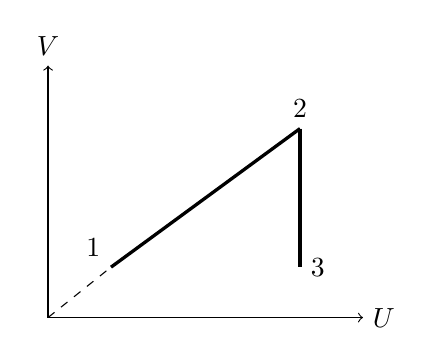
\begin{tikzpicture}[scale=0.8]
    \draw[->] (0,0) -- (5,0) node[right] {$U$};
    \draw[->] (0,0) -- (0,4) node[above] {$V$};

    % 1-2 to'g'ri chiziq (koordinata boshidan chiquvchi punktir bilan)
    \draw[dashed] (0,0) -- (1,0.8);
    \draw[very thick] (1,0.8) node[above left] {1} -- (4,3) node[above] {2};
    
    % 2-3 vertikal chiziq
    \draw[very thick] (4,3) -- (4,0.8) node[right] {3};
\end{tikzpicture}

\begin{enumerate}[label=\Alph*)]
\item o‘zgarmagan, ortgan
\item ortgan, kamaygan
\item pasaygan, ortgan
\item ortgan, ortgan

\end{enumerate}

\item Ideal gaz ustida grafikda ko‘rsatilganidek ikki xil izotermik jarayon bajarildi. Birinchi holda gazning ichki energiyasi $111$ kJ ni tashkil etgan. Ikkinchi holda esa birinchisidan $37$ kJ ga farq qilgan. Agar ikkala jarayondagi temperaturalar farqi $125$ K ni tashkil qilgan bo‘lsa, ikkinchi holdagi temperaturani (K) aniqlang.

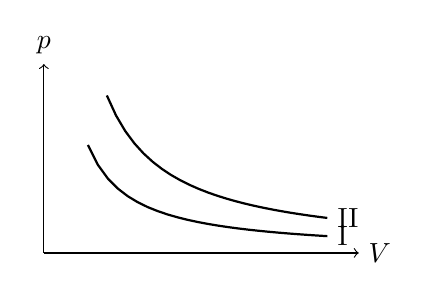
\begin{tikzpicture}[scale=0.8]
    \draw[->] (0,0) -- (5,0) node[right] {$V$};
    \draw[->] (0,0) -- (0,3) node[above] {$p$};

    % Ikkita giperbola
    \draw[thick, domain=0.7:4.5] plot (\x, {1.2/\x}) node[right] {I};
    \draw[thick, domain=1:4.5] plot (\x, {2.5/\x}) node[right] {II};
\end{tikzpicture}

\begin{enumerate}[label=\Alph*)]
\item 227
\item 375
\item 250
\item 500

\end{enumerate}

\item Bir xil miqdorda olingan H$_2$, O$_2$, N$_2$ gazlarining temperaturasi bir xil orttirilsa, qaysi gazning ichki energiyasi ko‘proq o‘zgaradi?
\begin{enumerate}[label=\Alph*)]
\item H$_2$
\item O$_2$
\item N$_2$
\item barchasiniki bir xil o‘zgaradi

\end{enumerate}

\item Gaz bosimini ifodalovchi quyidagi munosabatlarning qaysi biri to‘g‘ri emas?
\begin{enumerate}[label=\Alph*)]
\item $p=nkT$
\item $p=\dfrac{2}{3}nE_k$
\item $p=\dfrac{1}{2}\rho v_{kv}^2$
\item $p=\dfrac{2U}{3V}$

\end{enumerate}

\item Izobarik qizdirilgan bir atomli gazning ichki energiyasi qanday o‘zgaradi?
\begin{enumerate}[label=\Alph*)]
\item o‘zgarmaydi
\item kamayadi
\item ortadi
\item istalgancha o‘zgarishi mumkin

\end{enumerate}

\item Izobarik kengayganida ideal gazning ichki energiyasi qanday o‘zgaradi?
\begin{enumerate}[label=\Alph*)]
\item o‘zgarmaydi
\item kamayadi
\item ortadi
\item javob bosimga bog‘liq

\end{enumerate}

\item Izobarik siqilganda ideal gazning ichki energiyasi qanday o‘zgaradi?
\begin{enumerate}[label=\Alph*)]
\item o‘zgarmaydi
\item kamayadi
\item ortadi
\item ideal gazning ichki energiyasi hamma vaqt nolga teng

\end{enumerate}

\item Grafikda tasvirlangan jarayonda ideal gazning ichki energiyasi ...

\begin{tikzpicture}[scale=0.6]
    \draw[->] (0,0) -- (4,0) node[right] {$p$};
    \draw[->] (0,0) -- (0,4) node[above] {$V$};
    \node at (-0.2,-0.2) {$O$};

    % 1-2 vertikal chiziq (strelka bilan)
    \draw[very thick] (2,0.8) node[left] {1} -- (2,3.2) node[left] {2};
    \draw[->, very thick] (2,0.8) -- (2,2.2);
\end{tikzpicture}

\begin{enumerate}[label=\Alph*)]
\item oldin ortadi, keyin kamayadi
\item ortadi
\item kamayadi
\item o‘zgarmaydi

\end{enumerate}


\item Agar ideal gaz bosimi va hajmi 2 marta oshsa, uning ichki energiyasi qanday o‘zgaradi?
\begin{enumerate}[label=\Alph*)]
\item 2 marta oshadi
\item 8 marta oshadi
\item 2 marta kamayadi
\item 4 marta oshadi
\end{enumerate}

\item Ideal gazning bosimi 2 marta ortsa va hajmi 2 marta kamaysa, uning ichki energiyasi qanday o‘zgaradi?
\begin{enumerate}[label=\Alph*)]
\item o‘zgarmaydi
\item 4 marta kamayadi
\item 4 marta ortadi
\item 2 marta kamayadi

\end{enumerate}

\item Ideal gazning bosimi 2 marta kamayib, hajmi 3 marta ortsa, uning ichki energiyasi qanday o‘zgaradi?
\begin{enumerate}[label=\Alph*)]
\item 6 marta kamayadi
\item 6 marta ortadi
\item 1,5 marta kamayadi
\item 1,5 marta ortadi

\end{enumerate}

\item Bir atomli ideal gazning bosimi 50\% kamayib, hajmi 2 marta oshsa, uning ichki energiyasi qanday o‘zgaradi?
\begin{enumerate}[label=\Alph*)]
\item o‘zgarmaydi
\item 4 marta kamayadi
\item 4 marta ortadi
\item 2 marta kamayadi

\end{enumerate}

\item Ideal gaz izoxorik ravishda sovitilganda ichki energiyasi 1,5 marta kamaygan. Uning hajmi qanday o‘zgargan?
\begin{enumerate}[label=\Alph*)]
\item o‘zgarmagan
\item 1,5 marta kamaygan
\item 2,25 marta kamaygan
\item 2,25 marta ortgan

\end{enumerate}

\item Bir atomli gazning hajmi 3 marta kamayganda, bosimi 50\% ga oshgan bo‘lsa, uning ichki energiyasi qanday o‘zgargan?
\begin{enumerate}[label=\Alph*)]
\item 3 marta oshgan
\item 2 marta kamaygan
\item 3 marta kamaygan
\item o‘zgarmagan

\end{enumerate}

\item Agar bir atomli ideal gazning bosimi 3 marta ortib, hajmi 2 marta kamaygan bo‘lsa, uning ichki energiyasi qanday o‘zgaradi? ($m=\text{const}$)
\begin{enumerate}[label=\Alph*)]
\item 6 marta oshadi
\item 3 marta oshadi
\item 3 marta kamayadi
\item 1,5 marta oshadi

\end{enumerate}

\item Og‘zi ochiq idish qizdirildi. Idish ichidagi havoning ichki energiyasi qanday o‘zgaradi?
\begin{enumerate}[label=\Alph*)]
\item ortadi
\item o‘zgarmaydi
\item avval kamayadi, keyin ortadi
\item kamayadi

\end{enumerate}

\item Xonada pechka yoqilganda, xonadagi havoning ichki energiyasi qanday o‘zgaradi?
\begin{enumerate}[label=\Alph*)]
\item kamayadi
\item ortadi
\item o‘zgarmaydi
\item tashqi muhit temperaturasiga bog‘liq
\end{enumerate}

\item Ballondagi gazning temperaturasi $100$ K ga ortganda, uning bosimi 2 marta oshgan bo‘lsa, ichki energiyasi necha marta ortgan?
\begin{enumerate}[label=\Alph*)]
\item 1,5
\item 2
\item 4
\item 25

\end{enumerate}

\item Agar ballondagi gazning 25\% chiqib ketishi natijasida temperatura 1,2 marta pasaysa, ichki energiya necha marta kamayadi?
\begin{enumerate}[label=\Alph*)]
\item 4,8
\item 3,2
\item 1,6
\item 2,4

\end{enumerate}

\item Ballondagi gazning yarmi chiqib ketganda, bosim 3 marta kamaygan bo‘lsa, gazning ichki energiyasi qanday o‘zgargan?
\begin{enumerate}[label=\Alph*)]
\item 1,5 marta kamaygan
\item 3 marta oshgan
\item 3 marta kamaygan
\item 1,5 marta oshgan

\end{enumerate}

\end{enumerate}



\begin{table}[!ht]
\centering
\begin{tabular}{|c|c|c|c|c|c|c|c|c|c|}
\hline
1a & 2b & 3a & 4d & 5c & 6b & 7d & 8b & 9c & 10d \\ \hline
11b & 12c & 13a & 14d & 15a & 16c & 17a & 18b & 19c & 20c \\ \hline
21c & 22a & 23c & 24d & 25c & 26d & 27d & 28a & 29a & 30d \\ \hline
31b & 32c & 33d & 34a & 35d & 36c & 37b & 38b & 39c & 40c \\ \hline
41d & 42d & 43d & 44c & 45c & 46c & 47b & 48b & 49d & 50a \\ \hline
51d & 52a & 53a & 54b & 55d & 56b & 57c & 58b & 59c & 60c \\ \hline
\end{tabular}
\end{table}